\documentclass[10pt,twocolumn]{article}
\usepackage[letterpaper,top=0.8in,bottom=0.85in,left=0.75in,right=0.75in,columnsep=0.25in]{geometry}
\usepackage{times}
\usepackage{amsmath,amssymb,graphicx,booktabs,tikz,microtype,caption}
\usepackage[hidelinks]{hyperref}
\usepackage[numbers,sort&compress]{natbib}
\usetikzlibrary{positioning,arrows.meta}
\graphicspath{{figures/}}
\captionsetup{font=small,labelfont=bf,skip=4pt}
\setlength{\bibsep}{1.5pt}
\renewcommand{\bibfont}{\footnotesize}
\newcommand{\Lpred}{\mathcal{L}_{\text{pred}}}

\title{\vspace{-1.5em}\Large\bfseries How Walls Enter a Pixel World Model: Latent Geometry in Mini-Golf}
\author{Ali Seifeldin\\ \normalsize COMP 765, McGill University, Fall 2026}
\date{}

\begin{document}
\maketitle
\vspace{-2.5em}
\begin{abstract}
\noindent LeWorldModel (LeWM) trains a joint-embedding world model from pixels with one prediction loss and one regularizer, then plans by minimizing Euclidean distance to a goal image in latent space. Recent studies report that this distance is a poor guide on a two-room task. We rebuild a small LeWM (1.9M parameters, about five minutes per model on a laptop) for a continuous mini-golf game and ask whether the problem holds there. Our expectation was wrong. Latent distance jumps sharply at walls the model was never told about, and planning with one step of lookahead sinks 100\% and 97\% of episodes on two wall courses, beating a planner with the true physics and a straight-line cost (73\% and 35\%). In an exploratory, post hoc analysis, the evidence favours walls entering the latent space through the transitions rather than the pixels. A wall drawn in every image but absent from the physics leaves no trace (wall gap 0.96, against 7.88 for a real wall), a wall that blocks without bouncing gives an intermediate 3.82, and weakening shots shrinks the effect (7.88, 4.04, 1.93). The result has limits. A pocket course still defeats planning (48\%), though there the limit is the learned predictor rather than the latent cost, which reaches 100\% with true dynamics. Our proposed improvement, Dyna-style value iteration on a graph of latent states, gave no clear benefit.
\end{abstract}

\section{Introduction}
A world model lets an agent try actions in imagination before acting. Joint-embedding predictive architectures (JEPAs) do this without reconstructing pixels, by predicting the embedding of the next observation. LeWorldModel \cite{maes2026lewm} is an appealingly simple recent example: it trains end to end from pixels with a prediction loss and a single regularizer, and it plans by searching for actions whose imagined outcome lies close to a goal image's embedding.

That last step assumes that straight-line distance in latent space means something. Several 2026 papers argue that it often does not: on a two-room navigation task, latent distance is a poor proxy for reachability \cite{you2026ngc,hu2026scale,li2026trm}, tracking path length only near the goal and creating false basins \cite{you2026ngc}. LeWM itself reaches 87\% there, below two baselines \cite{maes2026lewm}. Mini-golf is a natural place to examine this. Walls matter, the task is easy to inspect, and a single shot can travel far and rebound.

This project began as a tabular study of Dyna \cite{sutton1990dyna} and moved to LeWM to engage with current world-model research. We set out with one expectation and one proposal. \textbf{H1:} latent distance will ignore walls, so planning with it will fail on wall courses. \textbf{H2:} Dyna-style value iteration over a graph of latent states will repair this. The first experiments contradicted H1, which led to a third hypothesis formed after seeing data, and therefore exploratory. \textbf{H3:} walls enter the latent space through the dynamics, because shots that reach them are blocked or bounce.

Our contributions are modest but concrete: a compact, reproducible LeWM for a new domain; a controlled ghost-wall experiment and a matched wall-gap metric that separate what the model sees from what it can do; suggestive evidence that action scale shapes latent geometry; a factorial test locating a planning failure in the predictor rather than the cost; and an honest negative result for our graph planner.

\section{Related Work}
\paragraph{World models.} Ha and Schmidhuber trained controllers inside a learned model of the environment \cite{ha2018worldmodels}, and PlaNet showed that latent models learned from pixels support online planning \cite{hafner2019planet}. DreamerV3 trains policies on imagined latent trajectories across many domains \cite{hafner2025dreamerv3}; profiling it for the course's first assignment is part of what motivated this project. MuZero \cite{schrittwieser2020muzero} and TD-MPC2 \cite{hansen2024tdmpc2} learn models aimed at decision-relevant quantities, and PETS \cite{chua2018pets} plans through uncertainty-aware dynamics. Assignment~1 of this course also fitted a cart-pole model and used it for receding-horizon control, which is the same decision-time use of a model that LeWM makes, except that there the state was given rather than learned from pixels.

\paragraph{JEPAs.} I-JEPA predicts representations of masked image regions \cite{assran2023ijepa}, and V-JEPA~2 scales the idea to video and adds action-conditioned planning toward image goals \cite{assran2025vjepa2}. DINO-WM plans on frozen pretrained features \cite{zhou2025dinowm}. PLDM trains a latent dynamics model on reward-free offline data and introduced the two-room task \cite{sobal2025pldm}. A recent study ablates what makes such planners work \cite{terver2026jepawms}. LeWM \cite{maes2026lewm} removes target encoders and stop-gradients by using SIGReg, a regularizer from LeJEPA \cite{balestriero2025lejepa}.

\paragraph{Is latent distance a good cost?} This is the closest literature. You et al.\ report that LeWM's distance correlates with path length near the goal but not globally on two rooms (Spearman $-0.17$ overall; SCALE reports 0.41 under another protocol), and replace it with shortest paths on a nearest-neighbour graph of latents \cite{you2026ngc}. SCALE adds a loss aligning latent and task-state distances using privileged state \cite{hu2026scale}. TRM trains a small temporal cost head and controls for wall crossing \cite{li2026trm}, and temporal straightening penalizes curvature during training \cite{wang2026straightening}. We use the graph idea as a baseline, and our matched wall-gap metric follows the same-room versus across-wall logic of TRM. Our finding differs in emphasis: rather than repairing the distance, we ask when it is already wall-aware and why.

\paragraph{Graphs and Dyna.} SPTM builds topological maps from observations \cite{savinov2018sptm}, and Search on the Replay Buffer searches graphs weighted by learned values \cite{eysenbach2019sorb}. Quasimetric \cite{wang2023qrl} and contrastive \cite{eysenbach2022contrastive} methods learn goal-reaching distances directly. Dyna updates values from model-generated experience \cite{sutton1990dyna,sutton2018rl}, and its later variants generate short model rollouts from real states \cite{janner2019mbpo}. Barkley and Fridovich-Keil caution that such synthetic experience can hurt \cite{barkley2025stealing}.

\section{Method}
\subsection{LeWorldModel}
An encoder maps an image $o_t$ to $z_t$, and a predictor maps $(z_t,a_t)$ to $\hat z_{t+1}$. Both train jointly on
\begin{equation}
\mathcal{L}=\underbrace{\lVert \hat z_{t+1}-z_{t+1}\rVert_2^2}_{\Lpred}+\lambda\,\mathrm{SIGReg}(Z).
\end{equation}
Alone, $\Lpred$ has a trivial solution: a constant encoder predicts itself perfectly. SIGReg prevents this by pushing the batch of embeddings toward an isotropic Gaussian. Testing that in high dimension directly is hard, but by the Cram\'er--Wold theorem \cite{cramer1936theorems} a distribution is fixed by its one-dimensional projections. SIGReg therefore draws $M$ random unit directions $u_m$ and applies the Epps--Pulley statistic \cite{epps1983test} to each projection $h_m=Zu_m$:
\begin{equation}
\mathrm{SIGReg}(Z)=\frac{1}{M}\sum_{m=1}^{M}\int w(t)\,\bigl|\hat\varphi_{h_m}(t)-e^{-t^2/2}\bigr|^2\,dt,
\end{equation}
where $\hat\varphi$ is the empirical characteristic function and $w$ a Gaussian window. In code the integral runs over $t\in[0,3]$ using symmetry, and the result is multiplied by the number of embeddings. Planning uses the cross-entropy method (CEM) \cite{rubinstein1999cem}: sample action sequences, roll them out with the predictor, keep the best, refit, and repeat. The cost is $\lVert\hat z_H-z_g\rVert_2^2$, where $z_g$ encodes the goal image (Figure~\ref{fig:pipeline}). No reward is used at any stage.

\begin{figure}[t]
\centering
\begin{tikzpicture}[font=\footnotesize,node distance=0.45cm,
 b/.style={draw,rounded corners=2pt,minimum height=0.62cm,align=center,inner sep=2.5pt},
 a/.style={-{Stealth[length=4pt]},thick}]
\node[b] (o) {image\\$o_t$};
\node[b,right=of o] (e) {encoder};
\node[b,right=of e] (p) {predictor};
\node[b,right=of p] (c) {$\lVert\hat z-z_g\rVert^2$};
\node[b,above=0.28cm of p] (act) {shot $a_t$ from CEM};
\node[b,below=0.28cm of c] (g) {goal image};
\draw[a] (o)--(e); \draw[a] (e)--node[above]{$z_t$}(p); \draw[a] (p)--node[above]{$\hat z$}(c);
\draw[a] (act)--(p); \draw[a] (g)--(c);
\draw[a] (c.north) |- (act.east);
\end{tikzpicture}
\caption{Planning in latent space. The encoder sees only pixels, and the planner never touches the simulator until it commits to a shot.}
\label{fig:pipeline}
\end{figure}

\subsection{Mini-golf environment}
The ball moves in a unit square with friction, restitution 0.8 on axis-aligned walls, higher friction in sand, and a hole that captures slow balls. One interaction is one shot: a velocity vector in the unit disc is applied to a ball at rest, physics runs until it stops or sinks, and the observation is the resting $64\times64$ image. The four courses are \emph{Open} (no interior wall, one sand trap), \emph{Gate} (a wall with a gap at the top), \emph{Slalom} (two offset walls), and \emph{Pocket} (a U-shaped enclosure around the hole, open away from the start). Figure~\ref{fig:maps} shows them.

\subsection{Our adaptation}
Each model trains per course on 60,000 random shots from random resting positions: reward-free, offline, and without any access to wall coordinates. Every image shares one fixed background, so wall pixels carry no information that varies between samples. Table~\ref{tab:deviations} lists how we differ from LeWM. Where its paper and code disagree we follow the code, as with the SIGReg range and weight. Because a resting ball is fully observed, one frame suffices. We apply SIGReg to current and next embeddings together and do not double the trapezoid weights, so $\lambda$ is not strictly comparable with LeWM's. Training takes 4,000 steps at batch size 256, or four to five minutes on an Apple M4 GPU.

\begin{table}[t]
\centering\footnotesize
\begin{tabular}{@{}lll@{}}
\toprule
Item & LeWM & This project\\
\midrule
Encoder & ViT-Tiny & 4-layer CNN\\
Predictor & Transformer & 3-hidden-layer MLP\\
Parameters & about 15M & 1.9M\\
Image size & $224^2$ & $64^2$\\
History & 1 or 3 frames & 1 frame\\
Latent dimension & 192 & 32\\
CEM rounds & 10--30 & 6\\
Horizon & 5 & 1 (2, 3 tested)\\
Replanning & after 5 actions & every shot\\
CEM initial spread & variance 1 & std 0.7\\
Same values & \multicolumn{2}{l}{BatchNorm before SIGReg, $M{=}1024$, 17 knots,}\\
 & \multicolumn{2}{l}{range $[0,3]$, $\lambda{=}0.09$, 300 samples, 30 elites}\\
\bottomrule
\end{tabular}
\caption{Differences from LeWM \cite{maes2026lewm} and its public code.}
\label{tab:deviations}
\end{table}

BatchNorm mattered. Our first version omitted it and collapsed to a constant encoder. A likely cause is visible in Equation~2: at an all-zero embedding the gradient of the characteristic-function term vanishes, and a ball changing only about 15 of 4,096 pixels makes that state easy to reach. Normalizing the projection head removed this constant collapse, though not the low-rank failure seen at small $\lambda$ below.

\subsection{Shot graph planner}
Our proposal adapts Dyna to the latent space. We cluster latents into 300 states with $k$-means. Each transition adds a directed edge between clusters, taken either from stored shots (\emph{replay}) or from the predictor applied to random shots (\emph{model}). Value iteration from the goal's cluster gives shots-to-go, $V(c)=\min_{c'}\,[\,1+V(c')\,]$, and CEM then minimizes $V$ at the imagined outcome instead of latent distance, using a soft average over the four nearest clusters and a small distance term to break ties. This is value iteration on a fixed graph, so it borrows Dyna's use of model transitions for planning but not its loop between acting and learning. Unlike the nearest-neighbour graph \cite{you2026ngc}, whose edges mean ``these embeddings are similar'', our edges mean ``one shot does this'', so a wall appears as a missing edge.

\subsection{Measuring walls in latent space}
\label{sec:gap}
We report Spearman correlation between latent distance to the goal and two references: straight-line distance and true path length from a shortest-path search. To target walls directly we define the \emph{wall gap}. We sample pairs of points 0.09 apart that straddle a wall, and compare the latent distance within each pair to the same pair slid along its own axis by one separation, so that it no longer straddles. Location and direction are thereby matched, and a value of 1 means the wall is invisible. Our first two versions of this metric were misleading: one confounded location and direction, and the other counted points outside the arena as free. Sanity checks on the open course and the ghost wall exposed these. The final metric reads 1.00 for a stand-in whose latent is the ball position, but this is only a sanity check, since any isometric latent gives exactly 1. We revised the metric after seeing the ghost result, so the ghost value is not an independent test of it.

\section{Experiments}
We train three seeds per course and evaluate each planner for 20 episodes per seed, from the course start and 19 random positions shared across planners, with a limit of 10 shots. Uncertainty is the standard deviation over the three seeds, which are the replication unit. With so few seeds we treat small differences as unresolved and run no significance tests.

\emph{Baselines} are random shots; \emph{aim}, which shoots straight at the hole; and CEM through the true physics with either a straight-line cost or a true path-length cost. The last is an oracle upper bound, and the pair shows how much the cost matters when the model is perfect. To separate model error from cost error for the learned planner, we also swap them one at a time: latent cost through the true physics, and true path length through the predictor, decoded with a linear probe. \emph{Latent planners} use latent L2 at horizons 1 to 3, with terminal cost as in LeWM, and an ``anytime'' variant at $H{=}3$ that scores a rollout by its best step. \emph{Graph planners} are our reimplementation of the nearest-neighbour graph \cite{you2026ngc} on 1,500 nodes, our shot graph in both forms, and a post hoc variant that switches to latent L2 when within about one shot of the goal.

\emph{Controls.} For the \emph{ghost wall}, the Gate wall is drawn identically in every image but removed from the physics. For the \emph{dead wall}, it blocks the ball with restitution 0, so it stops motion without a rebound. For \emph{shot power}, we scale all shots to 1/2 and 1/4 of their velocity, with shot limits of 20 and 40. We also vary $\lambda$ and dataset size, each on Gate with two seeds.

\section{Results}
\begin{figure*}[t]
\centering
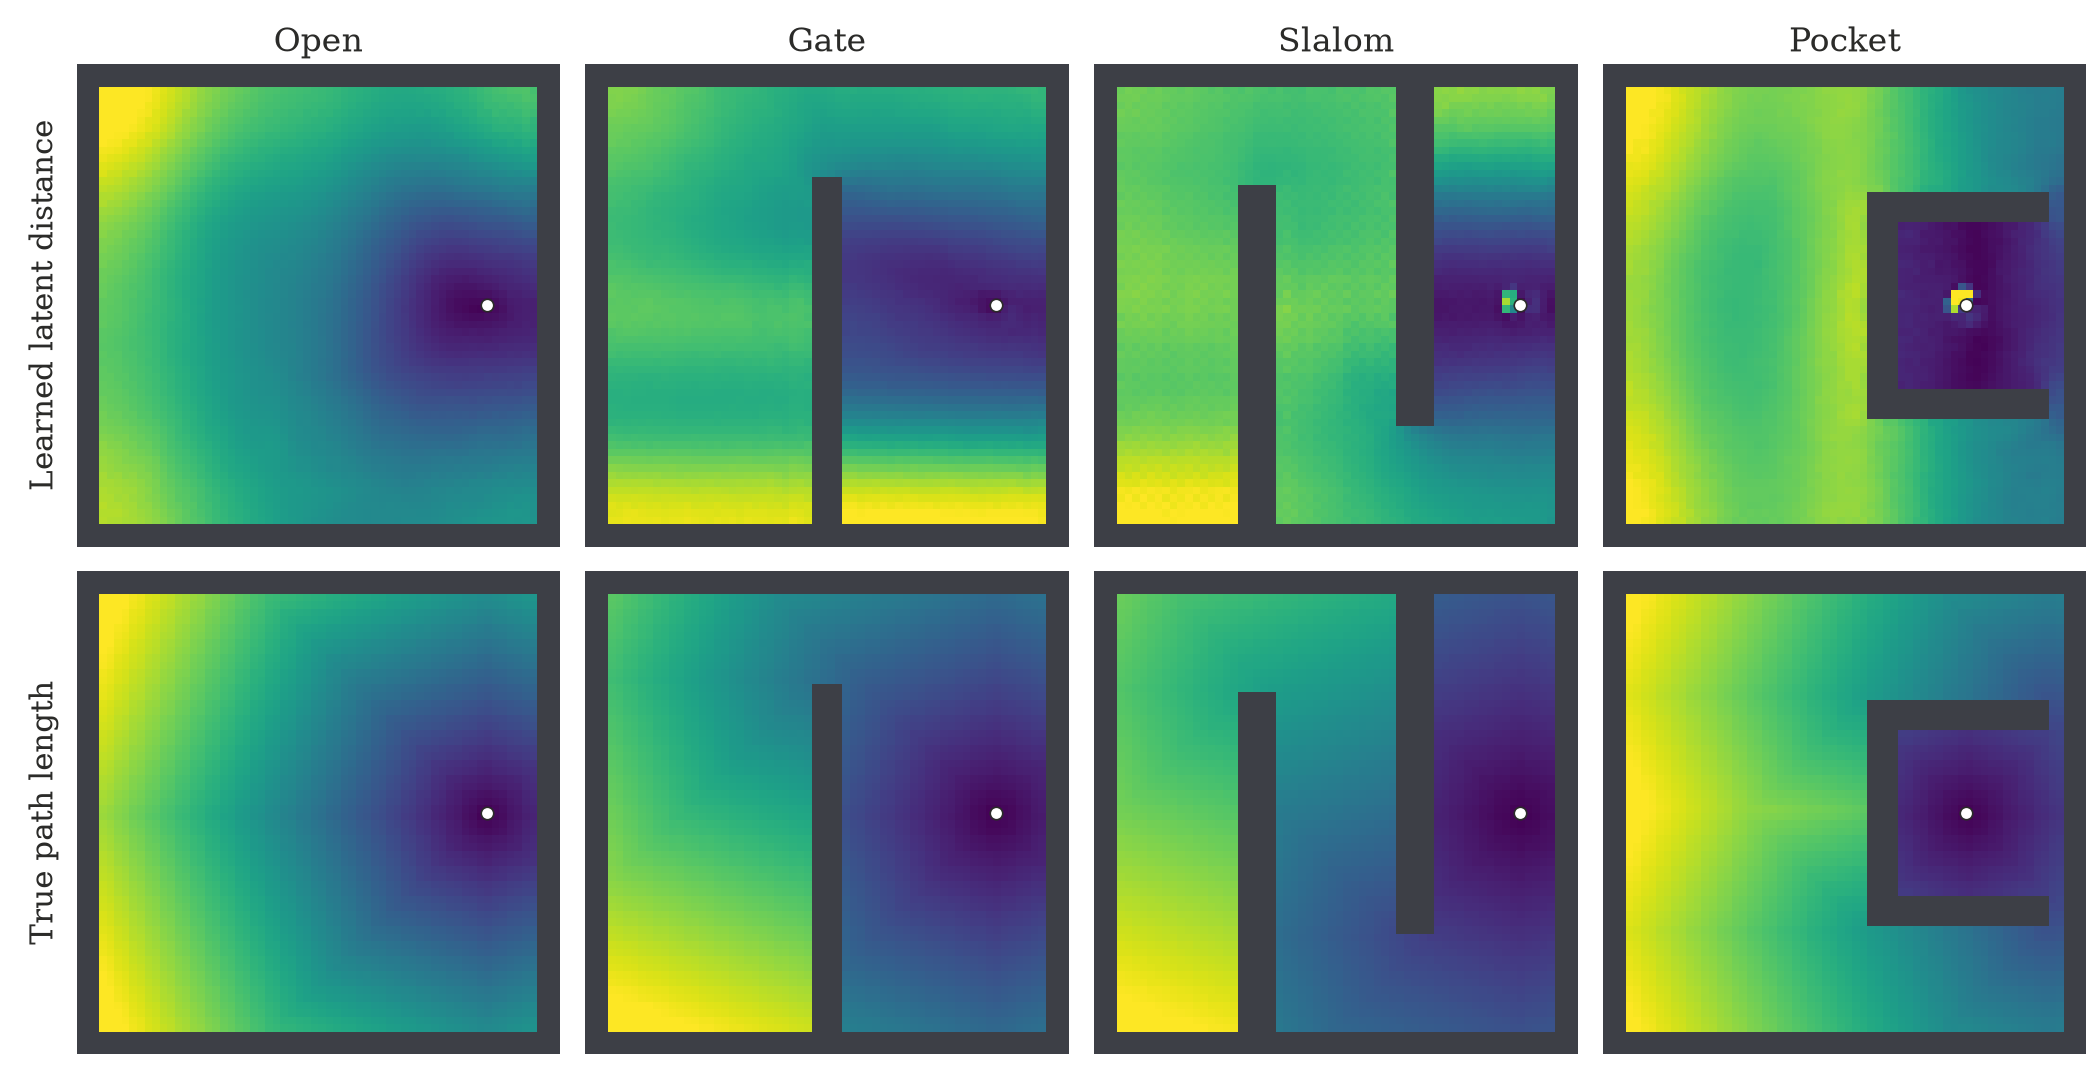
\includegraphics[width=0.86\textwidth]{distance_maps.png}
\caption{What the model learned (top) against the truth (bottom), seed 0. Colour is distance to the hole (white dot), dark for near and bright for far. Dark grey cells are solid. No wall positions were provided, yet the learned distance changes abruptly across walls. Small bright patches next to the hole lie where a shot never ends.}
\label{fig:maps}
\end{figure*}

\begin{table*}[t]
\centering\small
\begin{tabular}{@{}lcccc@{}}
\toprule
Planner & Open & Gate & Slalom & Pocket\\
\midrule
Random & $0.13\pm0.10$ & $0.13\pm0.15$ & $0.15\pm0.05$ & $0.07\pm0.03$\\
Aim at hole & $1.00\pm0.00$ & $0.47\pm0.16$ & $0.27\pm0.13$ & $0.10\pm0.05$\\
True physics, straight-line cost & $1.00\pm0.00$ & $0.73\pm0.10$ & $0.35\pm0.13$ & $0.40\pm0.26$\\
True physics, path-length cost (oracle) & $1.00\pm0.00$ & $1.00\pm0.00$ & $1.00\pm0.00$ & $1.00\pm0.00$\\
\midrule
Latent L2, $H{=}1$ & $0.93\pm0.12$ & $1.00\pm0.00$ & $0.97\pm0.06$ & $0.48\pm0.06$\\
Latent L2, $H{=}2$ & $0.47\pm0.29$ & $0.42\pm0.38$ & $0.55\pm0.09$ & $0.45\pm0.13$\\
Latent L2, $H{=}3$ & $0.20\pm0.05$ & $0.17\pm0.08$ & $0.38\pm0.15$ & $0.32\pm0.26$\\
Latent L2 anytime, $H{=}3$ & $0.95\pm0.09$ & $1.00\pm0.00$ & $0.98\pm0.03$ & $0.28\pm0.10$\\
\midrule
Nearest-neighbour graph \cite{you2026ngc} & $0.95\pm0.05$ & $1.00\pm0.00$ & $1.00\pm0.00$ & $0.48\pm0.34$\\
Shot graph, replay edges (ours) & $0.62\pm0.33$ & $0.87\pm0.19$ & $0.98\pm0.03$ & $0.57\pm0.20$\\
Shot graph, model edges (ours) & $0.60\pm0.35$ & $0.82\pm0.20$ & $1.00\pm0.00$ & $0.55\pm0.23$\\
Shot graph + L2 finish (ours, post hoc) & $0.92\pm0.10$ & $1.00\pm0.00$ & $1.00\pm0.00$ & $0.40\pm0.26$\\
\bottomrule
\end{tabular}
\caption{Fraction of episodes sunk within 10 shots (mean $\pm$ SD over three model seeds, 20 episodes each).}
\label{tab:planners}
\end{table*}

\subsection{A small model learns the game}
A linear probe, fitted and scored on the same grid, recovers ball position with RMSE 0.01 to 0.03 of the course width, so the representation is informative. On Open, latent planning sinks 93\% of episodes (Table~\ref{tab:planners}).

\subsection{H1 is rejected on Gate and Slalom}
We expected latent planning to stall at walls. Instead, latent L2 with one step of lookahead sinks 100\% of episodes on Gate and 97\% on Slalom, taking 2.2 and 3.4 shots on average, close to the oracle. It clearly beats true physics with a straight-line cost (73\% and 35\%), even though that planner has a perfect model. Restricting to starts with no clear line to the hole makes the contrast sharper: latent L2 sinks 37 of 37 and 43 of 45, against 21 of 37 and 6 of 45. Figure~\ref{fig:maps} shows why: the learned distance changes sharply at walls, with large wall gaps ($7.88\pm0.99$ and $8.33\pm0.11$). Global Spearman correlation is less informative here, since straight-line distance and path length are themselves correlated at about 0.92 on these courses: latent distance correlates with path length at $0.79\pm0.01$ and $0.82\pm0.04$, and with straight-line distance at $0.77$ and $0.77$.

\subsection{H3: transitions, not pixels, reveal walls}
Since every image shares one background, walls could only reach the encoder through the dynamics or through the ball's position relative to wall pixels. The ghost wall tests this. It looks identical, yet the wall gap falls from $7.88\pm0.99$ to $0.96\pm0.01$, close to the no-wall value of 1 (Figure~\ref{fig:profile}). On Gate, then, appearance alone is not enough. The ghost also differs in the states it allows, since balls can rest on the strip. The dead wall shares the real wall's states and blocks shots without rebound, and it gives $3.82\pm0.22$. So blocking alone produces a clear effect, and bouncing roughly doubles it.

\begin{figure}[t]
\centering
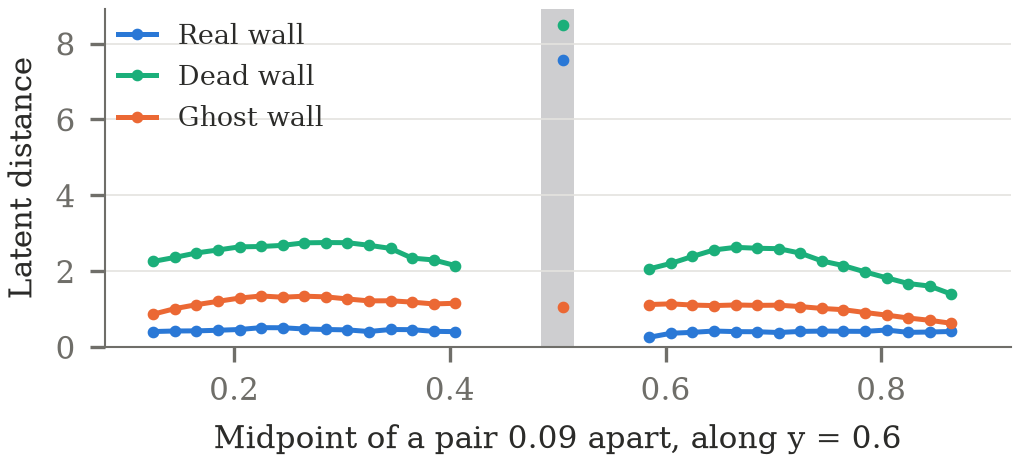
\includegraphics[width=\columnwidth]{wall_profile.png}
\caption{Latent distance between points 0.09 apart along a row crossing the Gate wall (grey), mean of three seeds. Pairs ending inside the wall are omitted. The real wall produces a large jump, the dead wall a smaller one, and the ghost none.}
\label{fig:profile}
\end{figure}

\begin{figure}[t]
\centering
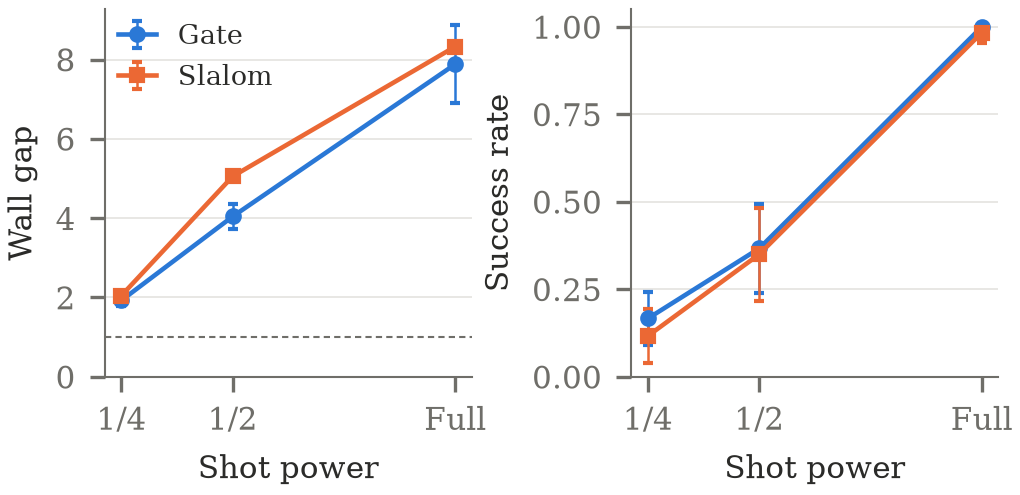
\includegraphics[width=\columnwidth]{power.png}
\caption{Weaker shots shrink the wall gap (left, dashed line marks no effect) and planning success (right). Mean and SD of three seeds. Range falls 16-fold at quarter power, while the shot limit grows only 4-fold. Full-power success was re-evaluated here with a different random stream, so Slalom reads 0.98 against 0.97 in Table~\ref{tab:planners}.}
\label{fig:power}
\end{figure}

Shot power then varies how much of the data involves walls, with the start distribution held fixed: an interior wall changes the outcome of 23\%, 7\%, and 2\% of random shots on Gate at full, half, and quarter power, and 42\%, 13\%, and 3\% on Slalom. The wall gap falls with it, to 7.88, 4.04, and 1.93 on Gate and 8.33, 5.05, and 2.05 on Slalom (Figure~\ref{fig:power}). This also argues against missing states as the whole explanation of the ghost result. Range shrinks 4 and 16 times as well, however, so the two effects are confounded.

The sweep offers a possible link to two-room results. As shots weaken, correlation with path length near the hole \emph{rises} on Gate (0.70, 0.95, 0.97) while global correlation collapses (0.79, 0.51, 0.17). Slalom follows at quarter power (0.96 near, 0.22 global), though less so at half power (0.67). This resembles the near-goal pattern reported by You et al.\ \cite{you2026ngc}. We did not run that benchmark, so the link remains a hypothesis. Weakening shots also does more than hide walls: correlation with \emph{both} path length and straight-line distance falls to about 0.2, and success (17\% and 12\%) partly reflects one-step lookahead that can only see a short distance, and a shot limit that grew by 4 while range fell by 16.

\subsection{Limits of latent L2}
\paragraph{Pocket.} Latent L2 sinks only 48\% here, and 0 of 3 from the course start, while the oracle reaches 100\%. The oracle changes both dynamics and cost, so Table~\ref{tab:factorial} swaps them one at a time. The same latent cost through the true physics sinks 100\%, whereas true path length through the predictor sinks only 53\%. The latent distance is therefore good enough here, as its wall gap suggests ($6.99\pm0.51$), and the bottleneck is prediction. Median one-shot error on shots affected by a wall is 0.074 on Pocket, against 0.041 for other shots, and 0.052 and 0.059 for wall shots on Gate and Slalom. The hole radius is 0.04. The same table supports the cost on Gate and Slalom too: it does well with either dynamics.

\begin{table}[t]
\centering\footnotesize
\begin{tabular}{@{}llccc@{}}
\toprule
Dynamics & Cost & Gate & Slalom & Pocket\\
\midrule
Predictor & Latent L2 & $1.00$ & $0.98$ & $0.50\pm0.18$\\
Predictor & Path length & $1.00$ & $0.88$ & $0.53\pm0.28$\\
True physics & Latent L2 & $0.95$ & $0.88$ & $1.00\pm0.00$\\
True physics & Shot graph & $0.93$ & $0.98$ & $0.92\pm0.10$\\
\bottomrule
\end{tabular}
\caption{Swapping dynamics and cost, $H{=}1$, mean over three seeds. The first row repeats Table~\ref{tab:planners}'s planner with a different random stream.}
\label{tab:factorial}
\end{table}

\paragraph{Horizon.} Longer terminal-cost planning is much worse (47\% and 20\% on Open at $H{=}2$ and 3). One untested explanation is specific to golf: a plan that sinks early must still end at the goal after its remaining shots, and errors compound. The anytime cost recovers most of this on three courses (95\%, 100\%, 98\%), which suggests the terminal formulation is the main problem there, though it uses more shots.

\paragraph{Ablations.} On Gate, 20,000 shots match 60,000 (100\%), and 5,000 remain usable (93\%). At $\lambda{=}1$ success stays at 95\% but the wall gap drops to $2.57\pm0.11$ and path-length correlation to $0.54\pm0.03$, possibly because a stronger Gaussian target flattens the geometry. Wall gap therefore does not predict planning success on its own: half-power models have a larger gap (4.04) and far lower success (37\%). At $\lambda{=}0.01$ the two seeds split. One failed entirely (0\%, gap 0.50), and the other gave the largest gap and correlation of any Gate model (25.2 and 0.90, 100\%). Both have low-dimensional latents (effective rank 1.2 and 2.2, against 6.8 at the default and 20 at $\lambda{=}1$), so this is a dimensional collapse that BatchNorm does not prevent. Two seeds cannot characterize it.

\subsection{H2 is not supported}
Our shot graph did not clearly improve on latent L2. On Pocket it reached $0.57\pm0.20$ against $0.48\pm0.06$, a difference well within seed variation. On Open it was clearly worse ($0.62$ against $0.93$), possibly because clusters are too coarse to aim the final shot. Adding a latent L2 finish repaired Open, Gate, and Slalom but not Pocket ($0.40\pm0.26$). The nearest-neighbour graph did about as well as anything, and replay and model edges did not differ noticeably. The graph is not simply broken: with true dynamics it reaches 92\% on Pocket (Table~\ref{tab:factorial}). But latent L2 reaches 100\% there, so even with a perfect predictor the graph shows no advantage. Latent distance already holds the information we built the graph to add.

\section{Discussion}
The central lesson is that latent geometry reflects the transitions a model is trained on. Our results suggest that a wall enters this model as a discontinuity in what shots can do, rather than as a visual object, and that it appears more strongly when more of the data reveals it. This suggests a practical point for JEPA planners: action scale and data coverage may affect whether a latent distance is usable, a different lever from the training-time and planning-time fixes in recent work \cite{you2026ngc,hu2026scale,li2026trm,wang2026straightening}. It also suggests checking where a failure lies before fixing it. We assumed Pocket needed a better cost and built one, but the factorial test shows it needed better prediction. The earlier tabular phase of this project found a similar pattern in an exploratory study: much of Dyna-Q's apparent gain on short routes depended on an optimistic initial value table, and an ordering between planning budgets turned out to be five-seed noise.

The natural next step is better prediction of wall contact. Shots touching a wall are a minority of the data and are predicted worse, so targeted data collection near failures, in the spirit of Dyna's loop between acting and learning, could help directly. Resampling wall-contact shots is a cheap first test. A second step is a direct test of the proposed link to earlier work, by running the shot-power sweep on a two-room task.

\section{Limitations}
Everything here is one small simulator with four hand-built courses and three seeds, and Pocket and the ablations carry wide uncertainty. Models are per course, so they do not test generalization to new layouts. The ghost and dead walls use Gate only. Our model is much smaller than LeWM and differs in architecture and history, so results may not transfer, and we did not reproduce any of LeWM's benchmarks. H3, the controls, and the wall-gap metric were developed after seeing results, and the metric has no independent validation. The dead wall gives a state-matched comparison, but no experiment fully separates blocked transitions from missing states. The goal is always the hole, unlike the varied goals in LeWM's evaluation. Finally, LeWM and several comparison papers are recent preprints, and their reported numbers come from different protocols.

\section{Conclusion}
We rebuilt LeWorldModel at a small scale for mini-golf, expecting its latent distance to fail at walls. On two of three wall courses it did not. Exploratory controls suggest why: a model trained on shots that are blocked by walls builds them into its geometry, bounces roughly double the effect, a wall that only looks real leaves almost no mark, and weaker shots weaken it. On Pocket the planner still fails, but the fault lies mainly with the predictor: the same latent cost succeeds with true dynamics, and our Dyna-style graph did not help. Open questions are whether the action-scale effect holds on standard benchmarks, how to gather the rare transitions that a hard course needs, and whether better prediction of wall-contact shots can close the gap to the oracle.

\paragraph{Reflection.} I started this project with an old paper and a tabular grid, and moved to LeWorldModel to work on a current question. What taught me most was being wrong in useful ways. I expected latent distance to ignore walls because recent papers said so, and the first distance maps showed the opposite. The ghost wall was the most satisfying experiment, because a simple idea turned a story into something I could test. Checking the metric where it should read nothing also exposed two mistakes in it: an open course with no walls scored about 10, which was the warning I needed. I now trust a metric only after checking that it reads ``nothing'' when nothing is there. An independent review of my draft caught a bigger error. I had blamed Pocket on the cost, and one experiment I had not run showed the predictor was at fault, so now I change one thing at a time before naming a cause. It also pushed me to test bouncing directly, which showed my first title claimed too much. I was surprised by how much BatchNorm matters, since without it the model collapsed. My proposed improvement did not work, and writing that plainly was harder than I expected. The assumption that changed most is that I used to treat a representation as a property of the images. I now think of it as also a property of the actions in the data.

\paragraph{Reproducibility.} Code, result files, and the interactive demo are at \url{https://github.com/Bakalala/COMP765/tree/main/putt_world}.

\small
\bibliographystyle{plainnat}
\bibliography{references}
\end{document}
